	
	\subsection*{Partie A}
	
	On considère la fonction polynôme du second degré \(P\) définie sur \(\mathbb{R}\) par :
	
	\[
	P(x) = x^2 - 7x + 6.
	\]
	
	1. La somme des racines est égale à 7 et leur produit à 6 : il est à peu près évident que ces racines sont 1 et 6.
	
	Sinon, on peut calculer :
	\[
	\Delta = 7^2 - 4 \times 6 = 49 - 24 = 25 = 5^2 > 0.
	\]
	Les racines sont donc :
	\[
	x_1 = \dfrac{7 + 5}{2} = 6 \quad \text{et} \quad x_2 = \dfrac{7 - 5}{2} = 1.
	\]
	
	2. On sait que le trinôme est positif (signe du coefficient 1) sauf entre les racines 1 et 6.
		\begin{center}
		\begin{tikzpicture}[double distance=2pt]
			\tkzTabInit{$x$/1,$P(x)$/1}{$-\infty$,$1$,$6$, $+\infty$}
			\tkzTabLine{,+,z,-,z, +}
			%\tkzTabVar{+/,-/$-1$,+/}
		\end{tikzpicture}
	\end{center} 
	
	\subsection*{Partie B}
	
	\(f(x) = 2x^3 - 21x^2 + 36x\).
	
	1. La fonction polynôme est dérivable sur \(\mathbb{R}\) et sur cet ensemble :
	
	\[
	f'(x) = 3 \times 2x^2 - 2 \times 21x + 36 = 6x^2 - 42x + 36 = 6(x^2 - 7x + 6) = 6P(x).
	\]
	
	2. Comme 6 est positif, le signe de \(f'(x)\) est celui de \(P(x)\) et on a vu que ce polynôme est positif sauf sur l’intervalle \(\left]1 ; 6\right[\).\\
	\(f(1) = 2 - 21 + 36 = 17\)\\
	 \(f(6) = 2 \times 216 - 21 \times 36 + 36 \times 6 = 432 - 756 + 216 = 648 - 756 = -108\).
		\begin{center}
		\begin{tikzpicture}[double distance=2pt]
			\tkzTabInit{$x$/1,$f'(x)$/1,$f(x)$/2}{$-\infty$,$1$,$6$, $+\infty$}
			\tkzTabLine{,+,z,-,z, +}
			\tkzTabVar{-/,+/$17$,-/$-108$,+/}
		\end{tikzpicture}
	\end{center} 
	3. On sait qu’une équation de la tangente \(T\) est : \(y = f(3) + f'(3)(x - 3)\).
	
	Avec \(f(3) = 2 \times 3^3 - 21 \times 3^2 + 36 \times 3 = 54 - 189 + 108 = -27\) et
	
	\[
	f'(3) = 6 \times 3^2 - 42 \times 3 + 36 = 54 - 126 + 36 = -36,
	\]
	
	l’équation devient :
	
	\[
	y - (-27) = -36(x - 3) \quad \text{ou} \quad y = -36x + 108 - 27 \quad \text{et finalement} \quad y = -36x + 81.
	\]
	
